\chapter{Analýza funkcií a architektúr operačných systémov}

Práca je zameraná na operačný systém pre vstavané systémy. Rozbor funkcionality operačných systémov bude preto zameraný najmä na túto oblasť. Mnoho rysov je spoločných pre každý operačný systém. Medzi výrazné odlišnosti od klasického systému pre osobný počítač, patria najmä veľmi obmedzená dostupná pamäť a pokročilý systém prerušení. Od toho je závislý pohľad na celkovú architektúru systému. V jednoduchých aplikáciach je možné použiť udalostne riadený systém. Zložitejšie vyžadujú prístup deterministického plánovača a fronty úloh. Druhým pohľadom je množina poskytovaných funkcií systému. Oba pohľady sú aplikačne závislé. Užívateľ by mal starostlivo zvážiť všetky potrebné požiadavky a podľa nich zvoliť koncepciu systému.

\section{Popis funkcií operačného systému}

Cieľom operačného systému je zabezpečiť kvalitné, stabilné a prehľadné rozhranie pre aplikačnú časť. Konkrétna množina funkcií je plne závislá od aplikácie. Medzi najčastejšie funkcie operačného systému patria:
\begin{itemize}
	\item Správa procesov a pamäte
	\item Medziprocesorová komunikácia
	\item Zabezpečenie synchronizácie operácií
	\item Všeobecne dostupné API rozhranie
\end{itemize}
Z ďalších funkcií je možné uviesť niekoľko špeciálnych a nie všeobecne typických pre každý operačný systém :
\begin{itemize}
	\item Ochrana pamäte
	\item Preemptívny multitasking
	\item Splnenie podmienok reálneho času
	\item Správa napájania
	\item Užívateľské rozhranie (textové alebo grafické)
\end{itemize}

Pre osobné počítače je v poslednej dobe typické najmä pokročilé užívateľské rozhranie. Z bežne dostupných sú to XFCE, KDE, Gnome a Unity
 \cite{linux_gui}. V ich prípade je v popredí častá interakcia s užívateľom systému. Preto je veľká pozornosť venovaná práve tejto časti.


V prípade vstavaných systémov je snaha vývojárov vytvoriť stabilný systém, kde nebude treba takmer žiaden dodatočný zásah zo strany programátora alebo užívateľa (s výnimkou upgradu). Typickým príkladom je mp3 prehrávač. Jeho užívateľské rozhranie sa rozhodne nemôže rovnať s rozhraním pre osobný počítač. V rámci možností hardvéru a najmä ceny, však poskytuje užívateľovi všetky potrebné funkcie. 

Príkladom systému, ktorý nedisponuje užívateľským rozhraním, sú ethernetové prepínače. Jednoduchšie prepínače realizujú posielanie rámcov uložením do medzipamäte. Po prijatí celého rámca a vyhodnotení adresy, sa rámec pošle ďalej. Toto všetko nevyžaduje žiadnu kontrolu od užívateľa.

Takmer nevyhnutnou súčasťou systému je medziprocesorová komunikácia. Najjednoduhšou formou je zdieľaná pamäť. Od nej je možné odvodiť ďalšie, pokročilejšie formy, najmä systém správ. V prípade viacúlohového systému, treba zabezpečiť vyhradený prístup do pamäte, čo predstavuje ďalšiu funkcionalitu systému - mutexy a semafóry. Táto množina funkcií vytvára základný balík pre pokročilú prácu so systémom.



\subsection{Synchronizácia úloh}

Každý viacúlohový operačný systém sa stretne s problémom synchronizácie dvoch a viacerých úloh. Táto situácia nastáva, ak aspoň dve vlákna požadujú vyhradený prístup k prostriedku. Tým môže byť napr. periférna operácia. Je potrebné preto zabezpečiť, aby druhé vlákno dostalo prístup k prostriedku až keď prvé ukončilo prácu s týmto zdrojom. Situáciu využitím jednoduchého mutexu modeluje nasledujúca Petriho sieť \cite{operacni_systemi}.

\begin{figure}[ht]
\begin{center}
\begin{minipage}{1.1\linewidth}
\begin{center}

\begin{tikzpicture}[node distance=1.3cm,>=stealth',bend angle=45]

  \tikzstyle{place}=[circle,thick,draw=blue!75,fill=blue!20,minimum size=6mm]
  \tikzstyle{red place}=[place,draw=red!75,fill=red!20]
  \tikzstyle{transition}=[rectangle,thick,draw=black!75,
  			  fill=black!20,minimum size=4mm]

  \tikzstyle{every label}=[red]
  \tikzstyle{language}=[Slovak]
  \begin{scope}
    % First net
     \node at (0,0) [place, tokens=1] (p1)  [label=above:{vlákno 1}]           {};
     \node at (0,-3) [place] (ks1) [label=left:$KS1$]                      {};
     \node at (0,-6) [place] (p2)                  {};


     \node at (4,0) [place, tokens=1] (q1)   [label=above:{vlákno 2}]               {};
     \node at (4,-3) [place] (ks2) [label=right:$KS2$]                      {};
     \node at (4,-6) [place] (q2)                  {};

     \node at (2,-3) [place, tokens=1] (sm) [label=above:$mutex$]                      {};


    \node at (0,-1.5)[transition] (e2) [label=left:{vstup}]  {}
      edge [pre]                (p1)
      edge [pre,bend left]      (sm)
      edge [post]               (ks1);


    \node at (0,-4.5)[transition] (e3) [label=left:{výstup}] {}
      edge [pre          ]      (ks1)
      edge [post,bend right]    (sm) 
      edge [post]               (p2);


    \node at (4,-1.5)[transition] (f2) [label=right:{vstup}]  {}
      edge [pre]                (q1)
      edge [pre,bend right]      (sm)
      edge [post]               (ks2);


    \node at (4,-4.5)[transition] (f3) [label=right:{výstup}] {}
      edge [pre          ]      (ks2)
      edge [post,bend left]    (sm) 
      edge [post]               (q2);

 \end{scope}  



  \begin{pgfonlayer}{background}
    \filldraw [line width=4mm,join=round,black!10]
      (p1.north  -| ks1.east)  rectangle (p1.south  -| ks1.west) ;
  \end{pgfonlayer}
\end{tikzpicture}


\caption {Synchronizácia procesov pomocou mutexu}
\label{obr1}
\end{center}
\end{minipage}
\end{center}
\end{figure}

Znázornené sú dve vlákna. Každé má svoju kritickú sekciu CSn. Vďaka použitiu mutexu môže vstúpiť do kritickej sekcie práve jedno vlákno. 
Označenie mutex je typické pre tzv. binárny semafór. Používajú sa všade tam, kde prostriedok môže byť pridelený len jednému procesu. V opačnom prípade je možné použiť klasický počítací semafór.

Treba poznamenať, že v prípade použitia jednoduchého mikrokontroléra je možné na vstup a výstup z kritickej sekcie použiť zakázanie, resp. povolenie prerušenia. Čas kedy je prerušenie zakázané, však treba obmedziť na minimum, aby nedošlo k narušeniu podmienok reálneho času a žiadostí na obsluhu prerušení.



\newpage
Ďalším typickým problémom synchronizácie, je riešenie problému čitateľov a zapisovateľa. Niekoľko vlákien číta dáta zo spoločnej pamäte. Čítanie je nedeštruktívne, preto môže k tejto zdieľanej oblasti pristupovať viac vlákien súčasne. Úloha zapisovateľa je do spoločnej pamäte zapísať dáta. Požaduje sa vyhradený prístup - zápis musí prebehnúť atomicky. Počas zápisu nemá žiaden z čitateľov prístup k pamäti. Situáciu je opäť možné modelovať Petriho sieťou.

\begin{figure}[ht]
\begin{center}
\begin{minipage}{1.1\linewidth}
\begin{center}

\begin{tikzpicture}[node distance=1.3cm,>=stealth',bend angle=45,auto]

  \tikzstyle{place}=[circle,thick,draw=blue!75,fill=blue!20,minimum size=6mm]
  \tikzstyle{red place}=[place,draw=red!75,fill=red!20]
  \tikzstyle{transition}=[rectangle,thick,draw=black!75,
  			  fill=black!20,minimum size=4mm]

  \tikzstyle{every label}=[red]

  \begin{scope}
    % First net
     \node at (0,0) [place, tokens=1] (p1)  [label=above:{vlákno R1}]           {};
     \node at (0,-3) [place] (ks1) [label=left:{čítanie}]                      {};
     \node at (0,-6) [place] (p2)                  {};


     \node at (3,0) [place, tokens=1] (q1)   [label=above:{vlákno R2}]               {};
     \node at (3,-3) [place] (ks2) [label=right:{čítanie}]                      {};
     \node at (3,-6) [place] (q2)                  {};

     \node at (10,0) [place, tokens=1] (r1)   [label=above:{vlákno W}]               {};
     \node at (10,-3) [place] (ks3) [label=right:{zápis}]                      {};
     \node at (10,-6) [place] (r2)                  {};

     \node at (8,-3) [place, tokens=2] (sm) [label=left:{semafor}]                      {};


    \node at (0,-1.5)[transition] (e2) [label=left:{vstup}]  {}
      edge [pre]                (p1)
      edge [pre,bend left]      (sm)
      edge [post]               (ks1);


    \node at (0,-4.5)[transition] (e3) [label=left:{výstup}] {}
      edge [pre          ]      (ks1)
      edge [post,bend right]    (sm) 
      edge [post]               (p2);


    \node at (3,-1.5)[transition] (f2) [label=right:{vstup}]  {}
      edge [pre]                (q1)
      edge [pre,bend left]      (sm)
      edge [post]               (ks2);


    \node at (3,-4.5)[transition] (f3) [label=right:{výstup}] {}
      edge [pre          ]      (ks2)
      edge [post,bend right]    (sm) 
      edge [post]               (q2);



    \node at (10,-1.5)[transition] (g2) [label=right:{vstup}]  {}
      edge [pre]                (r1)
      edge [pre,bend right]      (sm) [label=left:$2$]
      edge [post]               (ks3);


    \node at (10,-4.5)[transition] (g3) [label=right:{výstup}] {}
      edge [pre          ]      (ks3)
      edge [post,bend left]    (sm)  [label=left:$2$]
      edge [post]               (r2);

 \end{scope}  



  \begin{pgfonlayer}{background}
    \filldraw [line width=4mm,join=round,black!10]
      (p1.north  -| ks1.east)  rectangle (p1.south  -| ks1.west) ;
  \end{pgfonlayer}
\end{tikzpicture}


\caption {Problém čitateľov a zapisovateľa}
\label{obr1}
\end{center}
\end{minipage}
\end{center}
\end{figure}

Čitateľmi sú vlákna R1 a R2. Vždy pri požiadavke na čítanie odoberie čitateľ práve jeden token - druhý ostáva voľný pre druhé vlákno. Zapisovateľ však pri požiadavke na zápis musí odobrať dva tokeny. Tak zabráni vstupu ľubovoľného z čitateľov do kritickej sekcie, prípadne aj ďalšiemu zapisovateľovi. Princíp riešenia je totiž možné rozšíriť na ľubovoľný počet zapisovateľov i čitateľov.
Z praktických aplikácií tohto problému je možné uviesť napr. databázové systémy alebo klient-server aplikácie. Princíp je použiteľný aj pri prúdovom spracovaní číslicového signálu, napr. s využitím viacjadrového mikroprocesora. Treba poznamenať, že uvedená Petriho sieť nie je najspravodlivejším riešením. Ak budú čitatelia neustále vyžadovať prístup k dátam, zapisovateľ nikdy nedostane možnosť vstúpiť do kritickej sekcie. Na riešenie tejto situácie je potrebné využiť pomocný synchronizačný prostriedok, prípadne správu, ktorá informuje čitateĺov o novo aktualizovaných dátach.


\newpage

\subsection{Posielanie správ}

Existuje niekoľko vzácnych prípadov, kedy sú vlákna natoľko nezávislé, že nemusia spolu komunikovať. Vo veľkej väčšine aplikácií je však medzivláknová komunikácia nevynutná. Pomáha najmä pri dekompozícií riešeného problému a jeho rozdeleniu medzi viacero vlákien. Poslanie správy možno modelovať na Petriho sieti :

\begin{figure}[ht]
\begin{center}
\begin{minipage}{1.1\linewidth}
\begin{center}

\begin{tikzpicture}[node distance=1.3cm,>=stealth',bend angle=45,auto]

  \tikzstyle{place}=[circle,thick,draw=blue!75,fill=blue!20,minimum size=6mm]
  \tikzstyle{red place}=[place,draw=red!75,fill=red!20]
  \tikzstyle{transition}=[rectangle,thick,draw=black!75,
  			  fill=black!20,minimum size=4mm]

  \tikzstyle{every label}=[red]

  \begin{scope}
    % First net
     \node at (0,0) [place, tokens=1] (p1)  [label=above:{vlákno 1}]           {};
     \node at (0,-3) [place] (ks1)                      {};
     \node at (0,-6) [place] (p2)                  {};


     \node at (4,0) [place, tokens=1] (q1)   [label=above:{vlákno 2}]               {};
     \node at (4,-3) [place] (ks2) [label=right:{príjem}]                      {};
     \node at (4,-6) [place] (q2)                  {};

     \node at (2,-3) [place, tokens=1] (sm) [label=below:{posielanie}]                      {};


    \node at (0,-1.5)[transition] (e2) [label=left:{poslanie správy}]  {}
      edge [pre]                (p1)
      edge [post]               (ks1);


    \node at (0,-4.5)[transition] (e3) [label=left:{hotovo}] {}
      edge [pre          ]      (ks1)
      edge [post,bend right]    (sm) 
      edge [post]               (p2);


    \node at (4,-1.5)[transition] (f2) [label=right:{prijatie správy}]  {}
      edge [pre]                (q1)
      edge [pre,bend right]      (sm)
      edge [post]               (ks2);


    \node at (4,-4.5)[transition] (f3) [label=right:{hotovo}] {}
      edge [pre          ]      (ks2)
      edge [post]               (q2);

 \end{scope}  



  \begin{pgfonlayer}{background}
    \filldraw [line width=4mm,join=round,black!10]
      (p1.north  -| ks1.east)  rectangle (p1.south  -| ks1.west) ;
  \end{pgfonlayer}
\end{tikzpicture}

\caption {Posielanie správ medzi procesmi}
\label{obr1}
\end{center}
\end{minipage}
\end{center}
\end{figure}


V tomto prípade je použité synchronné prijímanie správ. Vlákno 2 čaká kým nepríjme správu. Existujú situácie, kde je to nežiadúce. Vtedy vlákno podľa potreby kontroluje príznak prítomnosti správy. Operácia príjímania je v tom prípade neblokujúca.

\newpage
\section{Architektúra operačných systémov}

Pri analýze systému je dôležitý pohľad celkovej koncepcie riešenia. Patrí sem rozdelenie na jednotlivé moduly, ktoré bloky bežia v prostredí jadra a ako sú implementované služby systému. Z tohto hľadiska je možné operačné systémy rozdeliť na tri skupiny :
\begin{itemize}
	\item Monolytické jadro
	\item Hybridné jadro
	\item Mikro jadro
\end{itemize}


\begin{figure}[htbp]
\begin{center}
\begin{minipage}{1.1\linewidth}
\begin{center}
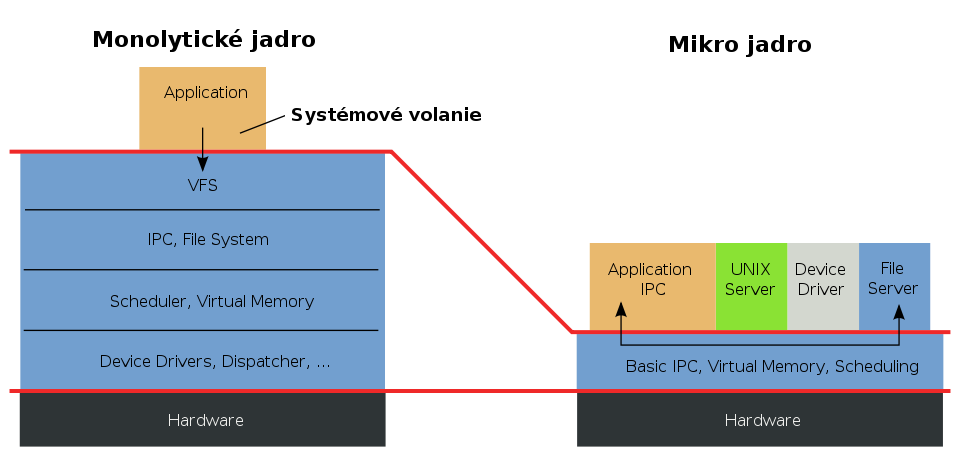
\includegraphics[width=0.8\textwidth]{images/os-structure_01.png}
\caption{Prehľad architektúr operačného systému}
\label{obr1}
\end{center}
\end{minipage}
\end{center}
\end{figure}


Nezávisle od aplikácie, je najdôležitejšou úlohou operačného systému správa procesov a prideľovanie procesorového času. Z pohľadu riešenia tejto časti (oblasť plánovača a prideľovania procesorového času) existujú systémy riadené striktne udalosťami, systémy spracovávajúce frontu úloh a samozrejme hybridné systémy. 

\begin{itemize}
	\item Udalostné systémy spúšťajú úlohy podľa výskytu udalostí - prerušenia alebo programovo generovaná udalosť. V princípe je to zovšeobecnenie systému prerušení pre akúkoľvek časť programu a nezávislosť od hardvéru. Táto koncepcia umožňuje realizovať systémy s krátkou dobou odozvy a výrazne šetrí pamäť.
	\item Systémy spracovávajúce frontu úloh poskytujú maximálnu robustnosť a flexibilitu. Typické sú pre ne pokročilé plánovacie algoritmy a prioritné prideľovanie zdrojov procesu.
	\item Hybridné riešenie kombinuje výhody oboch riešení.
\end{itemize}

\textbf{Monolitické jadro}
Tento model integruje všetky funkcie operačného systému do jedného bloku, tvoreného jadrom aj zvyškom systému. Volanie akejkoľvek funkcie systému je vždy realizované na úrovni jadra. Znižuje sa tak doba odozvy systému. Nevýhodou je narastajúca veľkosť jadra, aj čas strávený v priestore jadra. Mnohé moderné operačné sysemy (napr. Linux) riešia tento problém zavádzaním modulov do jadra až keď sú naozaj potrebné. Zvyšuje sa tak modularita systému. Typickými zástupcami sú Unix, Linux, FreeBSD, CP/M a MS-DOS. 

\textbf{Mikro jadro}
Jadro systému je minimalizované len na nevyhnutné funkcie - často len prepínanie úloh, správu pamäte a medziprocesorovú komunikáciu. Všetky ostatné služby sú riešené na aplikačnej úrovni. Často sa využíva model klient-server. Server je poskytovateľ služieb a beží ako samostatný proces. Klient požiada server o službu, komunikáciu sprostredkuje jadro. Systémy s týmto modelom sú veľmi robustné a spoľahlivé. Mnoho priemyselných aplikácií má práve túto architektúru. Nevýhodou môže byť dlhšia časová latencia na poskytnutie služby - systém ide vždy cestou : klient -> jadro -> server -> jadro -> klient. Typickými zástupcami sú QNX, Symbian OS, Phoenix-RTOS.

\textbf{Hybridné jadro}
Kombináciou výhod oboch prístupov vzniklo hybridné jadro. Časovo kritické a často volané služby bežia v prostedí jadra, ako v prípade monolytického systému. Služby nevyžadujúce rýchlu odozvu bežia ako jendotlivé servery. Príkladom je súborový systém, ktorý je relatívne pomalý voči ostatným službám. Najvýraznejším zástupcom v tejto kategórií je Windows NT.

\section{Klasifikácia systémov v závisloti na pricípe plánovania prepínania úloh}
\subsection{Udalostne riadené systémy}

Veľkú kategóriu operačných systémov vo vstavaných aplikáciach, tvoria systémy riadené udalosťami. Je to realizácia veľmi jednoduchej myšlienky : ak nie sú dáta, nie je čo robiť. Výrobcovia mikrokontrolérov si toto rýchlo uvedomili a vybavili mikrokontroléry pokročilým prerušovacím systémom. Táto koncepcia navyše umožňuje využiť režim zníženej spotreby - keď nie je udalosť, jadro procesora sa môže uspať.
Problematiku riadenia spotreby má veľmi dobre rozpracovanú firma Texas Instrumets so svojím 16 bitovým mikrokontrolérom s jadrom msp430 \cite {ti_msp430}.

Veľmi dobrou vlastnosťou tohto prístupu je spĺňanie podmienok reálneho času. To je veľmi dôležité hlavne v prípade číslicového spracovania signálu a v priemyselnom riadení. S využitím možností vnorených prerušení, je možné si poradiť aj s udalosťami vyskytujúcimi sa veľmi často (relatívne k času behu úloh - obsluhy prerušenia). Najlepšie situácu vystihne ukážka programu - blikanie led. Po reštarte treba inicializovať prerušenie od časovača a príslušný pin nastaviť ako výstup. Po povolení prerušení už nie je nutná účasť programu v hlavnej slučke - procesor je možné uspať a znížiť tak spotrebu. Vždy pri vyvolaní prerušovacej rutiny sa zmení stav na pine s led a vypne sa režim zníženej spotreby. Je vidieť, že v hlavnej slučke môže bežať ďalšia úloha.

{\small
\begin{verbatim}
int main()
{
 io_init();		  	  /*inicializácia hardvéru*/
 eint();			  /*globálne povolenie prerušení*/
 while (1)
  LPM0;				  /*vypnutie jadra procesora - zníženie spotreby*/
}

/*prerušenie časovača*/
interrupt(TIMER0_A0_VECTOR)  TIMER0_A0_ISR(void) 
{
 P1OUT^=0x01;	/*zmena stavu výstupu - led sa striedavo zapína a vypína*/
 LPM3_EXIT; 	/*znovu spustenie jadra po návrate z prerušenia*/
}
\end{verbatim}
}


Na pohľad vyzerá tento program veľmi jednoducho, ale má všetko potrebné pre reagovanie na jednoduchú udalosť. Veľký problém je hardvérová závislosť - prerušenia sú pevne zviazané s daným typom mikrokontroléra. Následne nie je možné program prenášať na iný mikrokontrolér. Problémom môže byť aj takmer nulová kontrola nad poradím a frekvenciou volaní prerušení. Riešením je vytvoriť programovú nadstavbu, ktorá zastreší systém prerušení aj systém volania udalostí. Princíp spočíva v minimalizácií programu v rutine obsluhy prerušenia - často stačí len nastavenie príznaku v globálnej premennej a okamžitý odchod z rutiny.

V anglickej literatúre sa tento princíp označuje ako event driven programming. Je to však pojem zaužívaný skôr pre programovanie osobných počítačov. Najčastejšie je tento princíp využívaný v spojení s grafickým rozhraním - kliknutie na tlačítko vyvolá udalosť OnClick. Operačný systém ju zachytí a pošle hlavnej slučke aplikácie. Samozrejmosťou je možnosť definovať vlastné udalosti. Treba poznamenať, že nad takouto správou udalostí beži pokročilý operačný systém. Možnosti realizovať to na mikrokontroléri bez preemptívneho multitaskingu však nič nebráni. 
V hlavnej slučke sa najprv overí fronta udalostí (zaslané prerušeniami alebo predošlými úlohami). Následne sa postupne vyberú a podľa adresy doručenia sa predávajú volaným úloham, napr. formou parametra funkcie.

Tento trend programovania je možné čoraz viac sledovať v mobilných zariadeniach \cite{android_event}. Aplikácia tak zbytočne nevyťažuje mikroprocesor a predlžuje sa životnosť batérie.

Priblíženie tohto populárneho spôsobu programovania na mikrokontroléroch, využila firma Quantum Leaps so svojim frameworkom QP \cite{qp_project}. Je to systém funkcií pre mikrokontroléry so veľmi odmedzenou kapacitou pamäťe. Projekt je založený na dekompozicií úlohy na stavové automaty. V hlavnej slučke programu sú v cykle spúšťané jednotlivé aktívne objekty. Existuje aj varianta pre populárnu vývojovú dosku Arduino. Projekt je uvoľnený ako Open Source pod GNU/GPL licenciou. V prípade problémov s touto licenciou (komerčná firma s inými požiadavkami), je možné vyjednať aj inú formu licencie.

Základným kameňom tohto projektu sú aktívne objekty. Výkonná časť algoritmu je realizovaná stavovým automatom. A objekty si medzi sebou vymieňajú dáta pomocou parametrov.

V nasledujúcej ukážke, je znázornený princíp objektov Qp. Úloha riešila problém obedujúcich filozofov. Jednotlivé časti problému boli rozdelené na niekoľko automatov (jednotlivé static QState Philo funkcie). Každá funkcia môže v sebe realizovať ďalší automat (podautomat, celkom nezávislý alebo jeden spoločný pre celý objekt).

{\small
\begin{verbatim}
typedef struct PhiloTag {
    QActive super;
} Philo;

static QState Philo_initial (Philo *me);
static QState Philo_thinking(Philo *me);
static QState Philo_hungry  (Philo *me);
static QState Philo_eating  (Philo *me);
\end{verbatim}
}

Vďaka princípu automatu môže zdanlivo paralelne bežať mnoho Qp objektov. Posielanie udalostí potom realizujú jednotlivé objekty. Systém Qp je tak vhodný pre riadenie procesov, nízkoenergetické aplikácie a mikrokontroléry s malým množstvom pamäte. Vďaka prehľadnému riešeniu rozdelením na objekty, umožňuje udržať prehľadnosť projektu a veľmi dobrú udržateľnosť produktu. K dispozícií je aj grafický nástroj na tvorbu systému.

Celkový pohľad na začlenenie Qp objektov v mikrokontroléri, znázorńuje nasledujúci obrázok. Je zrejmé, že systém Qp môže bežať pod kernelom iného operačného systému a tvoriť tak akýsi podsystém. V tom prípade sa však už zvýši doba odozvy, uplatnenie nájde aj v tejto podobe, napr. GUI pre riadenie dotykového displeja.

\subsection{Systémy s frontou úloh}

Veľkú skupinu operačných systémov tvorí klasický prístup k úlohovému spracovaniu. Je to najstaršia myšlienka využívaná už prvých zárodkoch operačných systémov. Tie jednoducho zoradili do fronty zoznam úloh a postupne ich spustili. Preempcia vtedy neexistovala, a tak úloha musela bez chyby zbehnúť, prípadne niekedy počas vykonávania predať riadenie opäť operačnému systému. Vznikali rôzne algoritmy ako zoradiť úlohy vo fronte, aby úlohy boli dokončené čo najoptimálnejšie - z hľadiska využitia procesora, aj z hľadiska spokojnosti užívateľa.
V navigačnom počítači Apolla bola použitá veľmi pokroková metóda plánovania - prioritné plánovanie. Je zrejmé, že systém navigácie lode spadá do kategórie tzv. mission critical systems. Preto boli úlohy so životne dôležitou funkciou vždy na začiatku fronty. Ak zostal po ich splnení procesorový čas, prešlo sa na spracovanie menej dôležitých úloh (chyba 1202 pri pristávaní Apolla 11). Všetky procesy ohľadom navigácie a stability lode však bolo potrebné plniť v prísne stanovených časových úsekoch. Ak nezostal čas na plnenie ďalšej menej dôležitej úlohy, úloha sa vôbec nezačala vykonávať - začal nový cyklus plánovača. Toto bol jeden z prvých systémov reálneho času a pravdepodobne prvý vstavaný systém na svete. Ešte dnes možno nájsť inšpiráciu vo vtedajšom prístupe k riešeniu. Problematike hardvéru aj softvéru počítača Apolla sa venuje \cite{apollo_agc}.

Nasledujúci program znázorňuje veľmi jednoduchý systém reálneho času, ktorý zabezpečuje periodické spúšťanie úloh.

{\small
\begin{verbatim}
/*ukazovateľ na funkciu a periodicita spúšťania*/
struct stCyclFunc {
		   u32 fFunc;
                   u32 bTimeStamp;
		  };

const stCyclFunc SYS_Active[] = { vTask1, 19,
				  vTask2,  0, 
				  vTask3,  0,
				  vTask4,  500 };
while(1) { /* hlavná slučka */
{
   if(SYS_stFlag.Timer1) /*čakanie na udalosť od časovača*/
    {
      SYS_stFlag.Timer1 = 0;
      for(i = 0; i < (sizeof(SYS_Active) / sizeof(stCyclFunc)); i++)
       {
        if(abActiveTick[i] == 0)  /*kontrola či časovač došiel k 0*/
         {
          abActiveTick[i] = SYS_Active[i].bTimeStamp;  /*čítač času opäť na vrchol*/
          SYS_Active[i].fFunc();  /*spustenie úlohy*/
         }
        else 
         abActiveTick[i]--; /*dekrementácia časových razítok
                                 pre každú nespustenú úlohu*/
      }
   }
}
\end{verbatim}
}

Je to jednoduchý nepreemptívny systém. Vždy pri tiku časovača sa dekrementuje počítadlo v každej úlohe. Úloha, ktorej počítadlo dosiahne hodnotu nula, bude spustená a počítadlo opäť nastavené na počiatočnú hodnotu. 

Rozšírením tejto koncepcie je možné vytvoriť plne univerzálny systém. V kombinácií s preemptívnym plánovaním nie je obmedzený blokovaním ostaných úloh inou, dlho bežiacou úlohou. 

